\section{Theorie}
\label{sec:Theorie}

\subsection{kosmische Myonen}
\label{subsec:kosmische Myonen}

Myonen sind instabile Elementarteilchen der Gruppe der Leptonen. 
Sie tragen ein negative Ladung, sind etwa 200-mal schwerer als Elektronen 
und haben eine Lebensdauer von ca. \qty{2,2}{\micro\second} \cite[125]{grupen}.
Sie entstehen durch die Wechselwirkung hochenergetischer kosmischer Strahlung
mit den oberen Schichten der Atmosphäre,
auch bekannt als sekundäre kosmische Strahlung.
Aus Protonenschauern gehen Pionen hervor,
die über die Zerfälle
\begin{equation*}
    \pi^{+} \rightarrow \mu^{+}+\nu_\mu \qquad \text {und} \qquad \pi^{-} \rightarrow \mu^{-}+\bar{\nu}_\mu
\end{equation*}
schließlich Myonen erzeugen \cite{demtroeder4}.


\subsection{Reichweite kosmischer Myonen}
\label{subsec:Reichweite kosmischer Myonen}

Nimmt man beispielsweise eine Energie von $E_\mu = \qty{10}{GeV}$ für kosmische Myonen 
und eine Ruheenergie von $E_0 = \qty{150e-3}{GeV}$ an,
so haben Myonen nach Eintreten in der Atmosphäre klassisch eine Reichweite von
\begin{equation}
    \begin{aligned}
    & s_{\text {klass }}=v \cdot \tau=c \sqrt{1-\left(\frac{E_0}{E_\mu}\right)^2} \cdot \tau \approx 660 \mathrm{~m}
    \end{aligned}
\end{equation}
Da sie sich jedoch mit relativistischen Geschwindigkeiten bewegen,
besitzen sie aufgrund von Längenkontraktion eine im Vergleich deutlich größere Reichweite von 
\begin{equation}
    \begin{aligned}
    & s_{\text {rel }}=v \cdot t^{\prime}=v \cdot \tau \gamma=v \cdot \tau\left(1-\left(\frac{v}{c}\right)^2\right)^{-\frac{1}{2}} \\
    & =c \sqrt{1-\left(\frac{E_0}{E_\mu}\right)^2} \cdot \frac{E_\mu}{E_0} \cdot \tau \approx 62854 \mathrm{~km} 
    \end{aligned}
\end{equation}
weswegen sie auch auf Meereshöhe mit einer Ereignisrate von $1 \, / \, 60\text{s} \, \text{cm}^2$ \cite[208]{grupen} messbar sind.


\subsection{Zerfallsgesetz}
\label{subsec:Zerfallsgesetz}

Die Lebensdauer eines instabilen Teilchens wird durch die Anzahl der Zerfälle pro Sekunde 
und pro Teilchen bestimmt, mit der es zerfällt. 
Sie folgt dem Zerfallsgesetz
\begin{equation} \label{eq:zerfallsgesetz}
    N(t) = N_0 \cdot \mathrm{e}^{-\lambda t} + U \, ,
\end{equation}
wobei $N_0$ die Anzahl der Anfangsteilchen, $\lambda$ die Zerfallskonstante
und $U$ Anzahl der Ereignisse der Untergrundstrahlung ist, 
welche hier das allgemeine Zerfallsgesetz modifizieren soll.
Diese berücksichtigt die Umgebungsradioaktivität und kosmische Strahlung.
Dabei stellt der Erwartungswert von $t$ die Lebensdauer $\tau$ dar und ergibt
\begin{equation} \label{eq:tau}
    \langle t\rangle=\tau=\int_0^{\infty} \lambda t \, \mathrm{e}^{-\lambda t} \mathrm{~d} t=\frac{1}{\lambda} \, ,
\end{equation}
siehe \cite{demtroeder4}. Um die in \autoref{eq:zerfallsgesetz} stehende Modifikation der Untergrundrate $U$ anzunähern,
wird ein Untergrundsignal als das Auftreffen eines zweiten Myons innerhalb der Suchzeit angenommen.
Diese Untergrundrate berücksichtigt jene Ereignisse, 
die nicht aus dem Zerfall hervorgehen und daher unerwünscht sind.
Unter der weiteren Annahme, 
dass die Wahrscheinlichkeit für dieses Ereignis poissonverteilt ist, 
ergibt sich die Anzahl der detektieren Myonen $n$ innerhalb der Suchzeit $T_\text{Such}$ zu
\begin{equation*}
    n=\frac{N_{0}}{T_{\text{Messung}}} \, ,
\end{equation*}
wobei $N_0$ die Anzahl der Startsignale und $T_{\text{Messung}}$ die Messzeit ist.
Mit dem Erwartungswert der gemessenen Ereignisse $T_\text{Such} \cdot n$ ergibt sich die Poissionverteilung zu
\begin{equation*}
    P(k)=\frac{\left(T_{\mathrm{Such}} \cdot n\right)^k}{k !} e^{T_{ \mathrm{Such}} \cdot n} \, .
\end{equation*}
Mithilfe der Wahrscheinlichkeit für ein weiteres Ereignis $P(1)$, 
kann die Anzahl der unerwünschten Ereignisse zu
\begin{equation*}
    N_{\mathrm{Fehl}}=N_{\mathrm{start}} \cdot P(1)
\end{equation*}
abgeschätzt werden.
Somit ergibt sich für ein Messkanal $N_\text{Kanal}$ die Untergrundrate
\begin{equation}\label{eq:untergrundrate}
    U=\frac{N_{\text {Fehl }}}{N_{\text {Kanal }}} \, .
\end{equation}


\subsection*{Bauteile}
% \label{sec:Bauteile}

In dem Folgenden werden die bei dem Versuch verwendeten Komponenten in ihrer prinzipiellen Funktionsweise erläutert.
\autoref{fig:schaltung} zeigt die Schaltung und die Bauteile.
\begin{figure}
    \centering
    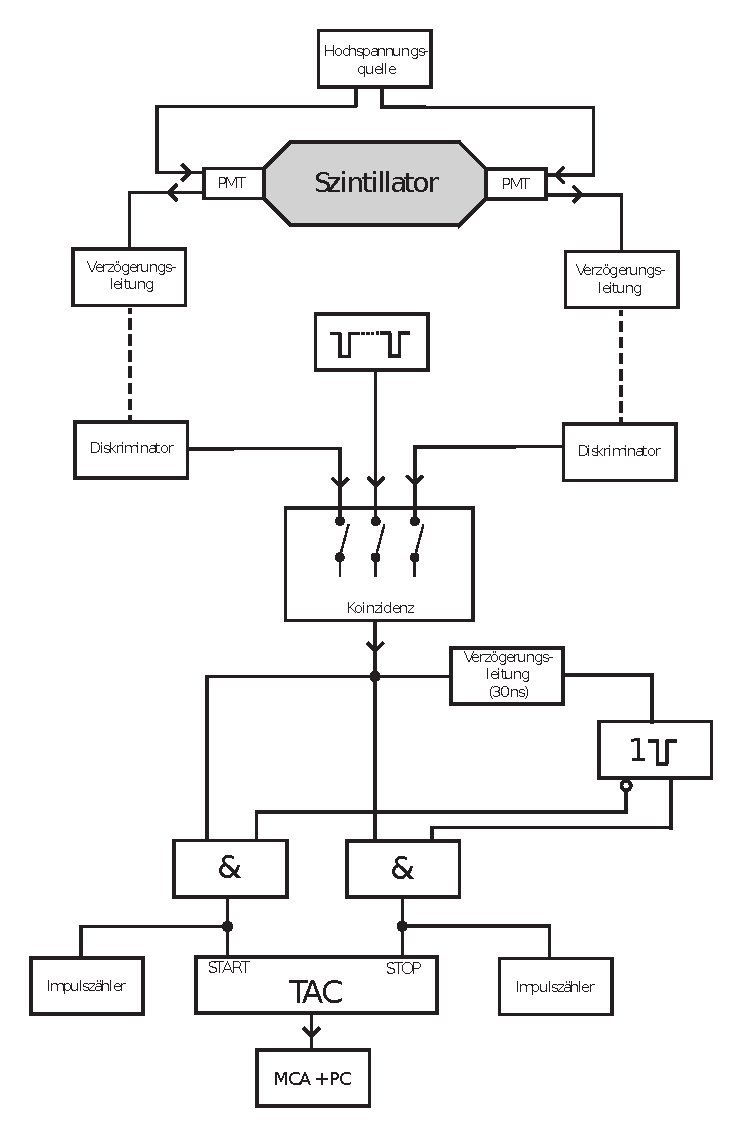
\includegraphics[width=0.8\textwidth]{pictures/schaltung.pdf}
    \caption{Blockschaltbild des Versuchsaufbaus \cite[3]{v01}.}
    \label{fig:schaltung}
\end{figure}


\subsubsection*{Photomultiplier}
Ein Photomultiplier (engl. \textit{photomultiplier tube}, PMT) ist ein Detektor, der in der Teilchenphysik, 
der Astronomie und anderen Bereichen eingesetzt wird, um einzelne Photonen zu erfassen und zu verstärken. 
Ein Photomultiplier ist eine Vakuumröhre, die schwache Lichtsignale misst. 
Sie enthält eine Photokathode, auf die eintreffende Photonen Elektronen auslösen. 
Diese Elektronen werden durch eine Spannung beschleunigt und treffen auf mehrere Elektrodenserien, 
die weitere Elektronen freisetzen. 
Dieser Prozess führt zu einer exponentiellen Verstärkung des Signals.
Bei der Messung der Lebensdauer kosmischer Myonen wird ein Photomultiplier verwendet, 
um das Lichtsignal zu registrieren, das entsteht, 
wenn ein Myon in einem Szintillationsdetektor zerfällt. 

\subsubsection*{Szintillationsdetektor}
Im Zusammenspiel mit zwei PMTs, ist ein Szintillator ein Detektor, der in der Lage ist, 
ionisierende Strahlung wie beispielsweise kosmische Strahlung zu detektieren. 
Es gibt verschiedene Arten von Szintillatoren wie organische und anorganische Szintillatoren,
die sich in ihrer Funktionsweise und ihrem Anwendungsgebiet unterscheiden.

Organische Szintillatoren bestehen aus organischen Materialen,
wie polymeren Festkörpern und Flüssigkeiten.
Die organischen Materialien funktionieren darüber, 
dass die Moleküle innerhalb des Materials durch die eingedrungenen Teilchen angeregt werden 
und bei Rückkehr in den Grundzustand ein Photon emittieren.
Die die Moleküle innerhalb des Materials werden durch die eingedrungenen Teilchen angeregt. 
Nach Abgabe eines Photons gehen die angeregten Moleküle wieder in den Grundzustand über.
Ein Vorteil dieses Materials besteht deswegen in der Zeitauflösung, 
während eine Energieauflösung aufgrund der breiten Frequenzmodenverteilung benachteiligt ist.
Diese Verteilung entsteht aufgrund verschiedener Schwingungsmoden im angeregten Zustand.

Anorganische Szintillatoren bestehen aus anorganischen Materialien wie Kristallen oder Keramik. 
Dabei ionisiert sich das Material und erzeugt ähnlich wie bei organischen Szintillatoren 
nach Rückkehr in den ursprünglichen energieärmeren Zustand ein Lichtsignal.
Anders als beim organischen Material, liegen hier diskrete Ionisationsenerigen vor,
weswegen eine höhere Energieauflösung möglich ist.

\subsubsection*{Verzögerungsleitung}
Die Verzögerungsleitungen gleichen Unterschiede in der Signalübermittlung aus
und werden durch anpassbare bzw. zuschaltbare Kabel realisiert.
Sie sind nötig, um eine präzise Synchronisation von Signalen zu ermöglichen
oder, wie in diesem Versuch, die Suchzeit durch Zeitverschiebung des Signals vorzugeben.

\subsubsection*{Diskriminator}
Das durch die Verzögerungsleitung gehende Signal wird durch Diskriminatoren geleitet.
Dabei wird das schwankende Signal der Photomultiplier ab einer gewissen Schwelle in diskrete
Ereignissignale umwandelt.

\subsubsection*{Koinzidenz}
Anschließend erreichen beide Signale eine Koinzidenzschaltung, welche ein Ausgangssignal
erzeugt, sobald zwei Photomultiplier gleichzeitig ein Signal aussenden.
Sie verwendet Verzögerungsleitungen, um die Signale zu synchronisieren, und eine Logikschaltung, 
um festzustellen, ob ein Zusammenfallen stattfindet.

\subsection*{Univibrator}
Der Univibrator, oder auch Monoflop bzw. monostabile Kippstufe genannt,
bleibt nach Eingang eines Signal nur für eine voreingestellte Zeit eingeschaltet
und wird durch eine Schaltung von Kondensatoren und Widerständen realisiert.

\subsection*{Time-Amplitude-Converter}
Nachdem die Signale die AND-Gatter passieren, 
gelangen sie zeitversetzt zum Time-Amplitude-Converter (TAC).
Dabei wird das Eingangssignal als Startsignal verwendet, 
um einen Ladevorgang eines Kondensators zu initiieren. 
Die Amplitude des geladenen Kondensators wird dann als Ausgangssignal des TAC verwendet, 
das proportional zur Dauer des Eingangssignals ist.

\subsection*{Multi-Channel-Analyzer}
Der Multi-Channel-Analyzer (MCA) oder Vielkanalanalysator ordnet mithile eines Computerprogramms 
die eingehenden Signale abhängig von ihrer Amplitude als Histogramm in Kanälen an.
Im Rahmen dieses Versuchs werden die Myonenereignisse gegen die Zeit aufgetragen.
Die erwartete Verteilung sollte eine charakteristische exponentielle Abnahme der Ereignisanzahl mit 
zunehmender Zeit aufgrund des exponentiellen Zerfalls der Myonen zeigen.